\documentclass[12pt]{article}
\usepackage{amsmath}
\usepackage{amsfonts}
\usepackage{amssymb}
\usepackage{graphicx}
\usepackage[a4paper, margin=0.98in]{geometry}
\usepackage{physics}
\usepackage{float}
\usepackage{booktabs}
\usepackage{makecell}
\usepackage{helvet}
\usepackage{fancyhdr}
\usepackage{titling}
\usepackage{longtable}
\usepackage{caption}
\usepackage{enumitem}
\usepackage{circuitikz}
\usepackage[hidelinks]{hyperref}
\usepackage{tikz}
\usepackage{subcaption}



% Define header
\pagestyle{fancy}
\fancyhf{}
\fancyhead[R]{PH3204: Electronics Laboratory}

% Title
\title{
  \vspace{-2cm}
  \Huge \textbf{PH3204: Electronics Laboratory} \\[0.4cm]
  \Large \textbf{Experiment 03:  Study of Operational Amplifier 
  (OpAmp) as inverting and non-inverting amplifier and
  its applications as adder and subtractor}
}

\author{
  \textbf{Ronit Bhuyan (22MS025)} \\[0.2cm]
  \textbf{Sub-Group B01}
}

\date{\today}

\begin{document}

\maketitle

\tableofcontents
\noindent\rule{\textwidth}{0.4pt}
\newpage

\section{Theory}


\subsection{Operational Amplifier (OpAmp)}
An Operational Amplifier or OpAmp is a differential amplifier that has a very high voltage gain, high input impedance and low output impedance. The OpAmp ha two inputs namely a non-inverting input($V_+$) and an inverting input($V_-$). The OpAmp amplifies the difference between the two inputs. The output voltage ($V_{out}$) is given by 
\begin{align*}
    V_{out} = A_0(V_+ - V_-)
\end{align*} 
where $A_0$ is the open loop gain of the amplifier. The OpAmp is usually operated with a negative feedback. The OpAmp used in this experiment is the LM741 OpAmp. The pin configuration of the LM741 OpAmp and its circuit diagram is shown in the figure below.




\begin{figure}[H]
\centering
\begin{minipage}{0.25\textwidth}
\centering
  



\tikzset{every picture/.style={line width=0.75pt}} %set default line width to 0.75pt        

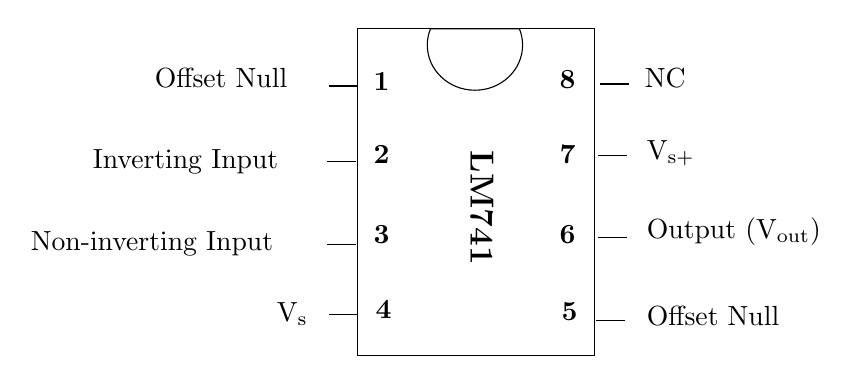
\begin{tikzpicture}[x=0.70pt,y=0.70pt,yscale=-1,xscale=1]
%uncomment if require: \path (0,300); %set diagram left start at 0, and has height of 300

%Shape: Rectangle [id:dp7033944784081119] 
\draw   (229,50.6) -- (351.2,50.6) -- (351.2,219.4) -- (229,219.4) -- cycle ;
%Shape: Chord [id:dp3994312770777564] 
\draw   (312.57,50.94) .. controls (313.62,53.53) and (314.2,56.35) .. (314.2,59.3) .. controls (314.2,72.17) and (303.19,82.6) .. (289.6,82.6) .. controls (276.01,82.6) and (265,72.17) .. (265,59.3) .. controls (265,56.35) and (265.58,53.53) .. (266.63,50.94) -- cycle ;
%Straight Lines [id:da12448979123953197] 
\draw    (214.2,80.4) -- (229.2,80.4) ;
%Straight Lines [id:da32433624264635386] 
\draw    (354.2,79.4) -- (369.2,79.4) ;
%Straight Lines [id:da4099130005520506] 
\draw    (214.2,198.4) -- (229.2,198.4) ;
%Straight Lines [id:da5527837141478477] 
\draw    (213.2,162.4) -- (228.2,162.4) ;
%Straight Lines [id:da7926452153091902] 
\draw    (213.2,119.4) -- (219.2,119.4) -- (228.2,119.4) ;
%Straight Lines [id:da3175360193460135] 
\draw    (352.2,201.4) -- (367.2,201.4) ;
%Straight Lines [id:da18341325604541547] 
\draw    (353.2,158.4) -- (368.2,158.4) ;
%Straight Lines [id:da46969219793073524] 
\draw    (353.2,116.4) -- (368.2,116.4) ;

% Text Node
\draw (300.5,112.5) node [anchor=north west][inner sep=0.75pt]  [rotate=-90] [align=left] {\textbf{{\large LM741}}};
% Text Node
\draw (236,72) node [anchor=north west][inner sep=0.75pt]   [align=left] {\textbf{1}};
% Text Node
\draw (237,190) node [anchor=north west][inner sep=0.75pt]   [align=left] {\textbf{4}};
% Text Node
\draw (236,151) node [anchor=north west][inner sep=0.75pt]   [align=left] {\textbf{3}};
% Text Node
\draw (236,110) node [anchor=north west][inner sep=0.75pt]   [align=left] {\textbf{2}};
% Text Node
\draw (333,191) node [anchor=north west][inner sep=0.75pt]   [align=left] {\textbf{5}};
% Text Node
\draw (332,151) node [anchor=north west][inner sep=0.75pt]   [align=left] {\textbf{6}};
% Text Node
\draw (332,110) node [anchor=north west][inner sep=0.75pt]   [align=left] {\textbf{7}};
% Text Node
\draw (332,71) node [anchor=north west][inner sep=0.75pt]   [align=left] {\textbf{8}};
% Text Node
\draw (123,70) node [anchor=north west][inner sep=0.75pt]   [align=left] {Offset Null};
% Text Node
\draw (91,112) node [anchor=north west][inner sep=0.75pt]   [align=left] {Inverting Input};
% Text Node
\draw (59,154) node [anchor=north west][inner sep=0.75pt]   [align=left] {Non-inverting Input};
% Text Node
\draw (90,189) node [anchor=north west][inner sep=0.75pt]   [align=left] {$ $};
% Text Node
\draw (186,191) node [anchor=north west][inner sep=0.75pt]   [align=left] {$\mathrm{V_{s}}$};
% Text Node
\draw (376,70) node [anchor=north west][inner sep=0.75pt]   [align=left] {NC};
% Text Node
\draw (377,107) node [anchor=north west][inner sep=0.75pt]   [align=left] {$\mathrm{V_{s+}}$};
% Text Node
\draw (377,150) node [anchor=north west][inner sep=0.75pt]   [align=left] {$ $};
% Text Node
\draw (377,147) node [anchor=north west][inner sep=0.75pt]   [align=left] {Output ($\mathrm{V_{out}})$};
% Text Node
\draw (377,193) node [anchor=north west][inner sep=0.75pt]   [align=left] {Offset Null};


\end{tikzpicture}

\end{minipage}
\hfill
\begin{minipage}{0.30\textwidth}
\centering






\tikzset{every picture/.style={line width=0.75pt}} %set default line width to 0.75pt        

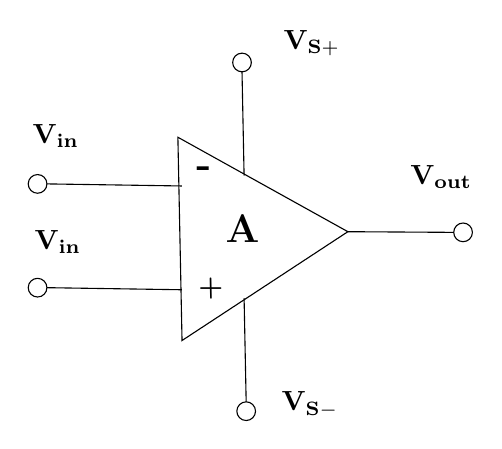
\begin{tikzpicture}[x=0.75pt,y=0.75pt,yscale=-1,xscale=1]
%uncomment if require: \path (0,300); %set diagram left start at 0, and has height of 300

%Flowchart: Extract [id:dp37966680550104925] 
\draw   (342.2,127.03) -- (262.3,179.46) -- (260.3,81.52) -- cycle ;
%Straight Lines [id:da7450651132831247] 
\draw    (197.2,104) -- (262.2,105) ;
%Straight Lines [id:da22744928578481094] 
\draw    (197.2,154) -- (262.2,155) ;
%Straight Lines [id:da9998583755076631] 
\draw    (342.2,127.03) -- (393.2,127.35) ;
%Straight Lines [id:da5159377376383624] 
\draw    (291.2,50) -- (292.2,100) ;
%Straight Lines [id:da38245740821617125] 
\draw    (292.2,159) -- (293.2,209) ;
%Shape: Circle [id:dp7432178640178844] 
\draw   (286.7,45.5) .. controls (286.7,43.01) and (288.71,41) .. (291.2,41) .. controls (293.69,41) and (295.7,43.01) .. (295.7,45.5) .. controls (295.7,47.99) and (293.69,50) .. (291.2,50) .. controls (288.71,50) and (286.7,47.99) .. (286.7,45.5) -- cycle ;
%Shape: Circle [id:dp8582173243755384] 
\draw   (288.7,213.5) .. controls (288.7,211.01) and (290.71,209) .. (293.2,209) .. controls (295.69,209) and (297.7,211.01) .. (297.7,213.5) .. controls (297.7,215.99) and (295.69,218) .. (293.2,218) .. controls (290.71,218) and (288.7,215.99) .. (288.7,213.5) -- cycle ;
%Shape: Circle [id:dp6580404394197098] 
\draw   (188.2,104) .. controls (188.2,101.51) and (190.21,99.5) .. (192.7,99.5) .. controls (195.19,99.5) and (197.2,101.51) .. (197.2,104) .. controls (197.2,106.49) and (195.19,108.5) .. (192.7,108.5) .. controls (190.21,108.5) and (188.2,106.49) .. (188.2,104) -- cycle ;
%Shape: Circle [id:dp4152539024478965] 
\draw   (188.2,154) .. controls (188.2,151.51) and (190.21,149.5) .. (192.7,149.5) .. controls (195.19,149.5) and (197.2,151.51) .. (197.2,154) .. controls (197.2,156.49) and (195.19,158.5) .. (192.7,158.5) .. controls (190.21,158.5) and (188.2,156.49) .. (188.2,154) -- cycle ;
%Shape: Circle [id:dp8877611769090077] 
\draw   (393.2,127.35) .. controls (393.2,124.86) and (395.21,122.85) .. (397.7,122.85) .. controls (400.19,122.85) and (402.2,124.86) .. (402.2,127.35) .. controls (402.2,129.84) and (400.19,131.85) .. (397.7,131.85) .. controls (395.21,131.85) and (393.2,129.84) .. (393.2,127.35) -- cycle ;

% Text Node
\draw (282,118) node [anchor=north west][inner sep=0.75pt]   [align=left] {\textbf{{\Large A}}};
% Text Node
\draw (189,74) node [anchor=north west][inner sep=0.75pt]   [align=left] {$\mathbf{V_{in}}$};
% Text Node
\draw (190,125) node [anchor=north west][inner sep=0.75pt]   [align=left] {$\mathbf{V_{in}}$};
% Text Node
\draw (371,94) node [anchor=north west][inner sep=0.75pt]   [align=left] {$\mathbf{V_{out}}$};
% Text Node
\draw (310,29) node [anchor=north west][inner sep=0.75pt]   [align=left] {$\mathbf{V_{S+}}$};
% Text Node
\draw (309,203) node [anchor=north west][inner sep=0.75pt]   [align=left] {$\mathbf{V_{S-}}$};
% Text Node
\draw (268,91) node [anchor=north west][inner sep=0.75pt]   [align=left] {\textbf{{\Large -}}};
% Text Node
\draw (268.85,148) node [anchor=north west][inner sep=0.75pt]  [xslant=-0.02] [align=left] {\textbf{+}};


\end{tikzpicture}

\end{minipage}
\\
\caption{\centering Pin configuration of LM741 OPAMP (left) and its circuit symbol (right)}
\end{figure}
\noindent
The OpAmp can be used in various configurations such as inverting amplifier, non-inverting amplifier, adder, subtractor,differentiator, integrator etc. In this experiment, we will study the OpAmp as an inverting amplifier, non-inverting amplifier, adder and subtractor.
\subsection{Inverting Amplifier}
The OpAmp can be used as an inverting amplifier by connecting it as per the following circuit diagram.
\begin{figure}[H]
  \begin{center}
    \begin{circuitikz}[american voltages,scale=1.2]
      \draw (0,0) node[op amp] (opamp) {}; %OpAmp

      \draw (opamp.-) to[R,l=$R_1$] ++(-2,0)  to [sV,l=$\mathrm{V_{in}}$] ++ (0,-2) node[ground]{}; 
      \draw (opamp.+) to[short] ++(0,-1) node[ground]{};
      %input

      \node[below] at (opamp.-) {\textbf{A}};

      
      %feedback loop
      \draw (opamp.-) to [short,*-] ++(0,1.1) to [R,l=$R_f$]++ (2,0) to [short,-*] (opamp.out);

      %output
      \draw (opamp.out) to [short,*-o] ++ (1,0) node[above]{$\mathrm{V_{out}}$};

      %power supply

      \draw (opamp.up) to[short,-*] ++(0,0.5) node[right]{$\mathrm{+15V}$};
      \draw (opamp.down) to[short,-*] ++(0,-0.5) node[right]{$\mathrm{-15V}$};


      
    \end{circuitikz}
  \end{center}
\label{fig:inverting_amp}
\caption{Circuit diagram of OpAmp as an Inverting Amplifier}
  
\end{figure}

\noindent
At the point \textbf{A}, the voltgae is 0 due to virtual ground. Theus, by applying Kirchoff's current law at the point \textbf{A}, we get 
\begin{align*}\label{eq:inverting}
  \frac{V_{in}-0}{R_1}= \frac{0-V_{out}}{R_f}
  \implies V_{out} = -\frac{R_f}{R_1}V_{in}
\end{align*}
Hence, the amplification $A_0$ in the case of inverting amplifier is given by
\begin{equation}\label{eq:inv}
  \boxed{
    A_0 = -\frac{R_f}{R_1}
  }
\end{equation}



\subsection{Non-Inverting Amplifier}
The circuit diagram of an OpAmp as a non-inverting amplifier is shown below.
\begin{figure}[H]
  \begin{center}
    \begin{circuitikz}[american voltages,scale=1.2]
      \draw (0,0) node[op amp] (opamp) {}; %OpAmp

      \draw (opamp.-) to[R,l=$R_1$] ++(-2,0) node[ground]{};
      \draw (opamp.+) to[sV,label=$\mathrm{V_{in}}$] ++(0,-2) node[ground]{};
      %input
      
      %feedback loop
      \draw (opamp.-) to [short,*-] ++(0,1.1) to [R,l=$R_f$]++ (2,0) to [short,-*] (opamp.out);

      %output
      \draw (opamp.out) to [short,*-o] ++ (1,0) node[above]{$\mathrm{V_{out}}$};

      %power supply
      \node[below] at (opamp.-) {\textbf{A}};


      \draw (opamp.up) to[short,-*] ++(0,0.5) node[right]{$\mathrm{+15V}$};
      \draw (opamp.down) to[short,-*] ++(0,-0.5) node[right]{$\mathrm{-15V}$};


      
    \end{circuitikz}
  
  \end{center}
\label{fig:non_inverting_amp}
\caption{Circuit diagram of OpAmp as a Non-Inverting Amplifier}
\end{figure}

\noindent
At point \textbf{A}, the potential is $V_{in}$. Thus, by applying Kirchoff's current law at point \textbf{A}, we get
\begin{align*}
  \frac{V_{in}-V_{out}}{R_1} = \frac{V_{out}-0}{R_f}
  \implies V_{out} = \left(1+\frac{R_f}{R_1}\right)V_{in}
\end{align*}
Hence, the amplification $A_0$ in the case of non-inverting amplifier is given by
\begin{equation}\label{eq:noninv}
  \boxed{
    A_0 = 1+\frac{R_f}{R_1}
  }
\end{equation}
  

\newpage
\subsection{Adder}
The OpAmp can be used as an adder by connecting it as per the following circuit diagram.
\begin{figure}[H]
  \begin{center}
    \begin{circuitikz}[american voltages,scale=1.2]
      \draw (0,0) node[op amp] (opamp) {}; %OpAmp
      
      %input
      \draw (opamp.-) -- ++(-1.5,0) coordinate (junction){};
      \draw (junction) -- ++(0,-1) to [R,l=$\mathrm{R_1}$,*-]++ (-2,0) node[above]{$\mathrm{V_1}$};
      \draw (junction) -- ++(0,0)to [R,l=$\mathrm{R_2}$,*-]++ (-2,0) node[above]{$\mathrm{V_2}$};
      \draw (junction) -- ++(0,+1)to [R,l=$\mathrm{R_3}$,*-]++ (-2,0) node[above]{$\mathrm{V_3}$};
      \draw (opamp.+) to[short] ++(0,-1) node[ground]{};
      
      
      %feedback loop
      \draw (opamp.-) to [short,*-] ++(0,1.1) to [R,l=$R_f$]++ (2,0) to [short,-*] (opamp.out);

      %output
      \draw (opamp.out) to [short,*-o] ++ (1,0) node[above]{$\mathrm{V_{out}}$};

      \node[below] at (opamp.-) {\textbf{A}};


      %power supply

      \draw (opamp.up) to[short,-*] ++(0,0.5) node[right]{$\mathrm{+15V}$};
      \draw (opamp.down) to[short,-*] ++(0,-0.5) node[right]{$\mathrm{-15V}$};


      
    \end{circuitikz}
\end{center}
\caption{Circuit diagram of OpAmp as an Adder}
\label{fig:adder}
\end{figure}
\noindent
Similar to the case of the inverting and non-inverting amplifiers, the potential at the point \textbf{A} is 0. Thus, by applying Kirchoff's current law at point \textbf{A}, we get
\begin{align*}
  \frac{0-V_1}{R_1}+\frac{0-V_2}{R_2}+\frac{0-V_3}{R_3} = \frac{V_{out}}{R_f}\\
  \implies V_{out} = -\left(\frac{R_f}{R_1}V_1+\frac{R_f}{R_2}V_2+\frac{R_f}{R_3}V_3\right)
\end{align*}
In the special case when $R_1=R_2=R_3=R_f=R$, the output voltage is given by
\begin{equation}\label{eq:add}
    \boxed{V_{out} = -(V_1+V_2+V_3)}
\end{equation}
Thus, the OpAmp acts as an adder in this case by addiing the input voltages.



\subsection{Subtractor}
The circuit diagram for OpAmp as a subtractor is shown below. 
\begin{figure}[H]
  \begin{center}
    \begin{circuitikz}[american voltages,scale=1.2]
      \draw (0,0) node[op amp] (opamp) {}; %OpAmp
      
      %input
      \draw (opamp.-) node{} to [R,label=$R_1$] ++(-4,0) to [sV,label=$\mathrm{V_1}$] ++(0,-3) node[ground]{};
      \draw (opamp.+) node{} to [R,label=$R_2$] ++(-2,0) to [sV,label=$\mathrm{V_2}$] ++(0,-2) node[ground]{};
      \draw(opamp.+) to [short] ++(0,-1) to [R,label=$R_0$] ++(0,-2) node[ground]{};
      
      %feedback loop
      \draw (opamp.-) to [short,*-] ++(0,1.1) to [R,l=$R_f$]++ (2,0) to [short,-*] (opamp.out);

      %output
      \draw (opamp.out) to [short,*-o] ++ (1,0) node[above]{$\mathrm{V_{out}}$};

      %power supply
      \node[below] at (opamp.-) {\textbf{A}};
      \node[below left] at (opamp.+) {\textbf{B}};


      \draw (opamp.up) to[short,-*] ++(0,0.5) node[right]{$\mathrm{+15V}$};
      \draw (opamp.down) to[short,-*] ++(0,-0.5) node[right]{$\mathrm{-15V}$};


      
    \end{circuitikz}
\end{center}
\caption{Circuit diagram of OpAmp as a Subtractor}
\label{fig:subs}
\end{figure}
\noindent
Again, by applying the concept of virtual ground, we know that the potntial at point $\textbf{A}$ and at the point $\textbf{B}$ is the same. Let the potential at point $\textbf{A}$ and $\textbf{B}$ be $V$. Thus, by applying Kirchoff's current law at point A, we get
\begin{align*}
  \frac{V-V_1}{R_1}=\frac{V_{out}-V}{R_f}
\end{align*}
Similarly, by applying Kirchoff's current law at point B, we get
\begin{align*}
  \frac{V-V_2}{R_2}=\frac{-V}{R_0}
\end{align*}
Solving for $V_{out}$, we get

\begin{align*}
  V_{out} = \frac{R_f}{R_1} \left(\frac{V_2 R_0}{R_0 + R_2} - V_1 \right) + \frac{V_2 R_0}{R_0 + R_2} 
\end{align*}
In the special case when $R_1=R_2=R_f=R_0=R$, the output voltage is given by
\begin{equation}\label{eq:sub}
 \boxed{ V_{out} = V_2 - V_1}
\end{equation}
Thus, the OpAmp acts as a subtractor in this case by subtracting the input voltages.



\section{Data and Analysis}
\subsection*{Inverting Amplifier}
Here, we present the data collected for the inverting amplifier for various combinations of $R_i$ and $R_f$. The data is presented below in Table \ref{tab:combined}.

\begin{table}[H]
  \centering
  \begin{subtable}{0.48\textwidth}
      \centering
      \begin{tabular}{|c| c| c|}
          \hline
          $V_{in}$ (V) & $V_{out}$ (V) & Amplification($A_0$) \\
          \hline
          1.00 & -2.20 & -2.20 \\
          2.00 & -4.38 & -2.19 \\
          3.00 & -6.57 & -2.19 \\
          4.00 & -8.75 & -2.19 \\
          5.00 & -10.93 & -2.19 \\
          \hline
          \multicolumn{3}{|c|} {Average $A_0$ = -2.19} \\
          \multicolumn{3}{|c|} {Theoretical Value = -2.18} \\
          \hline
      \end{tabular}
      \caption{$R_i=996\Omega, R_f=2170\Omega$}
      \label{tab:third}
  \end{subtable}
  \hfill
  \begin{subtable}{0.48\textwidth}
      \centering
      \begin{tabular}{|c| c| c|}
          \hline
          $V_{in}$ (V) & $V_{out}$ (V) & Amplification($A_0$) \\
          \hline
          0.02 & -0.18 & -9.00 \\
          0.20 & -2.03 & -10.15 \\
          0.40 & -4.04 & -10.10 \\
          0.60 & -6.01 & -10.02 \\
          0.79 & -7.95 & -10.06 \\
          \hline
          \multicolumn{3}{|c|}{Average $A_0$ = -9.87} \\
          \multicolumn{3}{|c|}{Theoretical Value = -9.89} \\
          \hline
      \end{tabular}
      \caption{$R_i=996\Omega, R_f=9850\Omega$}      
      \label{tab:second1}
  \end{subtable}
  
  \bigskip
  \bigskip

  \begin{subtable}{0.48\textwidth}
    \centering
    \begin{tabular}{|c|c|c|}
        \hline
        $V_{in}$ (V) & $V_{out}$ (V) & Amplification($A_0$) \\
        \hline
        0.50 & -2.30 & -4.60 \\
        1.00 & -4.59 & -4.59 \\
        1.50 & -6.85 & -4.57 \\
        2.00 & -9.16 & -4.58 \\
        2.50 & -11.44 & -4.58 \\
        \hline
        \multicolumn{3}{|c|}{Average $A_0$ = 4.58} \\
        \multicolumn{3}{|c|}{Theoretical Value = -4.56} \\
        \hline
    \end{tabular}
    \caption{$R_i=2160\Omega, R_f=9850\Omega$}
    \label{tab:first}
\end{subtable}
\hfill
\begin{subtable}{0.48\textwidth}
    \centering
    \begin{tabular}{|c|c|c|}
        \hline
        $V_{in}$ (V) & $V_{out}$ (V) & Amplification($A_0$) \\
        \hline
        2.00 & -0.90 & -0.45 \\
        4.00 & -1.80 & -0.45 \\
        6.00 & -2.71 & -0.45 \\
        8.00 & -3.62 & -0.45 \\
        10.00 & -4.53 & -0.45 \\
        \hline
        \multicolumn{3}{|c|}{Average $A_0$ = -0.45} \\
        \multicolumn{3}{|c|}{Theoretical Value = -0.45} \\
        \hline
    \end{tabular}
    \caption{$R_i=21800\Omega, R_f=9850\Omega$}
    \label{tab:second}
    \end{subtable}
  \caption{Data for Inverting Amplifier for various combinations of $R_i$ and $R_f$}
  \label{tab:combined}
\end{table}

\subsection*{Non-Inverting Amplifier}

Here, we present the data collected for the inverting amplifier for various combinations of $R_i$ and $R_f$. The data is presented below in Table \ref{tab:combined2}.

\begin{table}[H]
  \centering
  \begin{subtable}{0.48\textwidth}
      \centering
      \begin{tabular}{|c| c| c|}
          \hline
          $V_{in}$ (V) & $V_{out}$ (V) & Amplification($A_0$) \\
          \hline
          1.00 & 3.20 & 3.20 \\
          1.50 & 4.77 & 3.18 \\
          2.00 & 6.35 & 3.18 \\
          3.00 & 9.54 & 3.18 \\
          4.00 & 12.69 & 3.17 \\
          \hline
          \multicolumn{3}{|c|} {Average $A_0$ = 3.18} \\
          \multicolumn{3}{|c|}{Theoretical Value = 3.15} \\
          \hline
      \end{tabular}
      \caption{$R_i=1006\Omega, R_f=2160\Omega$}
  \end{subtable}
  \hfill
  \begin{subtable}{0.48\textwidth}
      \centering
      \begin{tabular}{|c| c| c|}
          \hline
          $V_{in}$ (V) & $V_{out}$ (V) & Amplification($A_0$) \\
          \hline
          1.00 & 2.02 & 2.02 \\
          2.00 & 4.04 & 2.02 \\
          3.00 & 6.07 & 2.02 \\
          4.00 & 8.10 & 2.03 \\
          5.00 & 10.10 & 2.02 \\
          \hline
          \multicolumn{3}{|c|}{Average $A_0$ = 2.02} \\
          \multicolumn{3}{|c|}{Theoretical Value = 2.00} \\
          \hline
      \end{tabular}
      \caption{$R_i=985\Omega, R_f=983\Omega$}      
  \end{subtable}
  
  \bigskip
  
  \begin{subtable}{0.48\textwidth}
    \centering
    \begin{tabular}{|c|c|c|}
        \hline
        $V_{in}$ (V) & $V_{out}$ (V) & Amplification($A_0$) \\
        \hline
        1.00 & 1.12 & 1.12 \\
        3.00 & 3.33 & 1.11 \\
        5.00 & 5.54 & 1.11 \\
        7.00 & 7.75 & 1.11 \\
        9.00 & 9.96 & 1.11 \\
        \hline
        \multicolumn{3}{|c|}{Average $A_0$ = 1.11} \\
        \multicolumn{3}{|c|}{Theoretical Value = 1.01} \\
        \hline
    \end{tabular}
    \caption{$R_i=21800\Omega, R_f=2170\Omega$}
\end{subtable}
\hfill
\begin{subtable}{0.48\textwidth}
    \centering
    \begin{tabular}{|c|c|c|}
        \hline
        $V_{in}$ (V) & $V_{out}$ (V) & Amplification($A_0$) \\
        \hline
        0.50 & 2.84 & 5.68 \\
        1.00 & 5.60 & 5.60 \\
        1.50 & 8.38 & 5.59 \\
        2.00 & 11.18 & 5.59 \\
        2.50 & 13.97 & 5.59 \\
        \hline
        \multicolumn{3}{|c|}{Average $A_0$ = 5.61} \\
        \multicolumn{3}{|c|}{Theoretical Value = 5.53} \\
        \hline
    \end{tabular}
    \caption{$R_i=2170\Omega, R_f=9850\Omega$}
\end{subtable}
  
  \caption{Data for Non-Inverting Amplifier for various combinations of $R_i$ and $R_f$}
  \label{tab:combined2}
\end{table}

\subsection*{Adder}

In this section, we present the data collected for the OpAmp as an adder for various combinations of $R_i$ and $R_f$. The data is presented below in Table \ref{tab:voltage_data_adder}.

\begin{table}[H]
    \centering
    \begin{tabular}{|c|c|c|c|c|}
        \hline
        $V_1$ (V) & $V_2$ (V) & $V_3$ (V) & $V_{out}(\text{Experimental})$ (V) & $V_{out}(\text{Theoretical})$ (V)  \\
        \hline
        0.72 & 1.02 & 1.45 & 3.15 & 3.19 \\
        1.44 & 1.73 & 2.92 & 6.01 & 6.09 \\
        1.27 & 1.99 & 2.04 & 5.23 & 5.30 \\
        1.52 & 1.31 & 2.16 & 4.92 & 4.99 \\
        1.40 & 1.40 & 2.81 & 5.55 & 5.61 \\
        1.78 & 1.67 & 3.01 & 6.34 & 6.46 \\
        0.41 & 0.45 & 0.82 & 1.66 & 1.68 \\
        0.52 & 0.74 & 1.05 & 2.26 & 2.31 \\
        1.65 & 2.75 & 3.31 & 7.52 & 7.71 \\
        1.11 & 1.85 & 2.23 & 5.03 & 5.19 \\
        \hline
    \end{tabular}
    \caption{OpAmp as an Adder}
    \label{tab:voltage_data_adder}
\end{table}


\subsection*{Subtractor}
Finally, we have tabulated the data collected for the OpAmp as a subtractor for various combinations of $R_i$ and $R_f$. The data is presented below in Table \ref{tab:voltage_data2}.

\begin{table}[H]
  \centering
  \begin{tabular}{|c|c|c|c|}
      \hline
      $V_1$ (V) & $V_2$ (V) & $V_{out}(\text{Experimental})$ (V) & $V_{out}(\text{Theoretical})$ (V) \\
      \hline
      3.60 & 4.80  & 1.14  & 1.20 \\
      2.55 & 3.18  & 0.60  & 0.63 \\
      0.82 & 3.55  & 2.68  & 2.73 \\
      5.18 & 6.93  & 1.65  & 1.75 \\
      6.67 & 8.91  & 2.12  & 2.24 \\
      0.46 & 0.61  & 0.15  & 0.15 \\
      1.93 & 2.58  & 0.63  & 0.65 \\
      3.61 & 4.85  & 1.19  & 1.24 \\
      4.57 & 5.55  & 0.95  & 0.98 \\
      9.02 & 12.03 & 2.85  & 3.01 \\
      \hline
  \end{tabular}
  \caption{OpAmp as a Subtractor}
  \label{tab:voltage_data2}
\end{table}

\section{Conclusions}
In this experiment, we have studied the use of an OpAmp as an amplifier (non-inverting and inverting) , adder and a subtractor. 
In case of the inverting and non-inverting amplifier, we experimented with the values of $R_i$ and $R_f$ and calculated the amplification factor $A_0$, which matched pretty well to the the theoretical value calculated using the equation \ref{eq:inv} and \ref{eq:noninv}.

\noindent
Similarly, for the adder and subtractor, we experimented with the values of $R_i$ and $R_f$ and calculated the output voltage $V_{out}$, which accurately matched to the the theoretical value calculated using the equation \ref{eq:add} and \ref{eq:sub}.



\section{Sources of Error}
\begin{itemize}
  \item There can be errors while measuring the resistance values of the resistors used in the circuit due to the internal resistances of the given multimeters. This can potentially lead to errors in the calculation of the amplification factor.
  \item Similarly, the may also be erros in the calculated values of the output voltage due to the internal resistance of the used multimeters.
\end{itemize}

\end{document}